\documentclass{article}
\usepackage{tikz}

\begin{document}

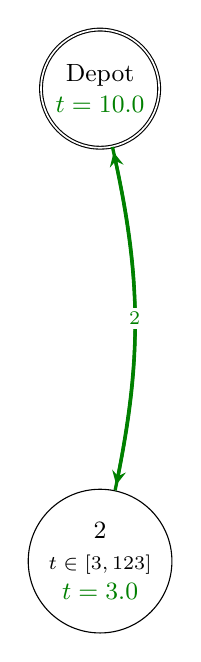
\begin{tikzpicture}[
    location/.style={
        circle,
        draw,
        minimum size=1.4cm,
        inner sep=2pt,
        align=center,
        font=\small
    },
    depot/.style={
        circle,
        draw,
        double,
        minimum size=1.5cm,
        inner sep=2pt,
        align=center,
        font=\small
    },
    solution/.style={
        ->,
        thick,
        green!50!black,
        >=stealth,
        line width=1.2pt,
        shorten >=2pt
    },
    possible/.style={
        -,
        dashed,
        gray
    },
    edge label/.style={
        fill=white,
        inner sep=1.5pt,
        font=\scriptsize
    }
]

\node[depot] (L1) at (0.0,3.0) {
    Depot\\
    {\color{green!50!black}$t=10.0$}
};

\node[location] (L2) at (-0.0,-3.0) {
    2\\
    {\scriptsize$t\in[3,123]$}\\
    {\color{green!50!black}$t=3.0$}
};

\draw[solution,bend left=12]
    (L1) to node[edge label] {2} (L2);

\draw[solution,bend right=12]
    (L2) to node[edge label] {2} (L1);

\end{tikzpicture}
\end{document}

